The quality of the predictions of the thermo-electrical model is affected by two major factors: First, there is the quality of the input parameters, and second there are errors introduced by reducing the complex 3D geometry into a linear thermal impedance network. The former have been discussed throughout this paper where the different inputs have been presented. For the latter we have studied the agreement of predictions from network model with the more accurate results obtained from FEA for selected states of the system.

For the verification of this agreement we have studied the sensor temperature curve for a barrel end-of-stave module up to thermal runaway. For this study we do not vary any of the input parameters in the model other than the sensor leakage power. We therefore can reduce the complex network to its Thevenin equivalent, which is identical to the network studied in ref.~\cite{Beck:2010zzd} and we use the analytical epxressions given there. The comparison of this prediction is shown in figure xxx. Despite a large temperature variation of about 15$^\circ$C across the sensor, which is caused by heat flux from the end-of-structure card and degraded thermal impedance at the end of the stave due to ceramic sections in the cooling pipe, the network model predicts the runaway within 1$^\circ$C of the result from the FEA. This agreement is not likely to significantly degrade the predictions beyond the errors introduced by uncertainties of other inputs to the model. 

\begin{figure}[ht]
\centering
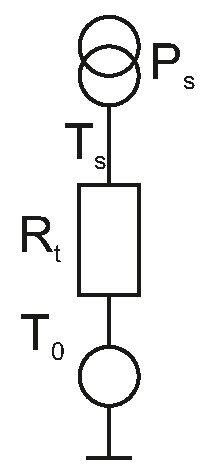
\includegraphics[width=0.1\linewidth]{figures/replacement.pdf}\quad\quad
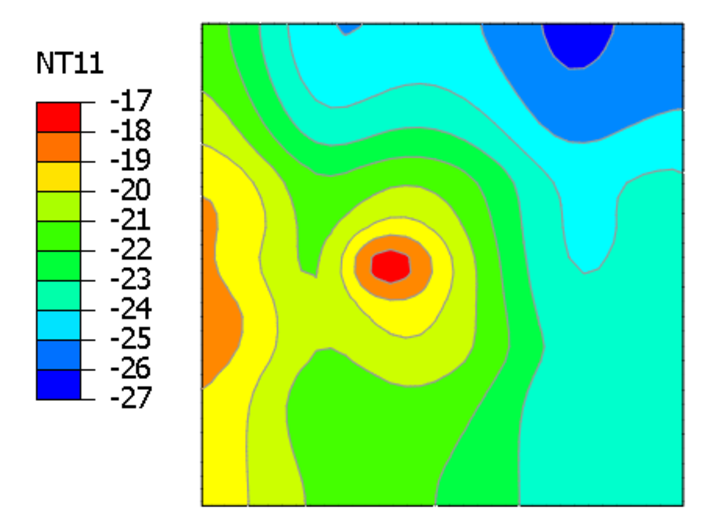
\includegraphics[width=0.25\linewidth]{figures/verificationFEA.pdf}\quad\quad
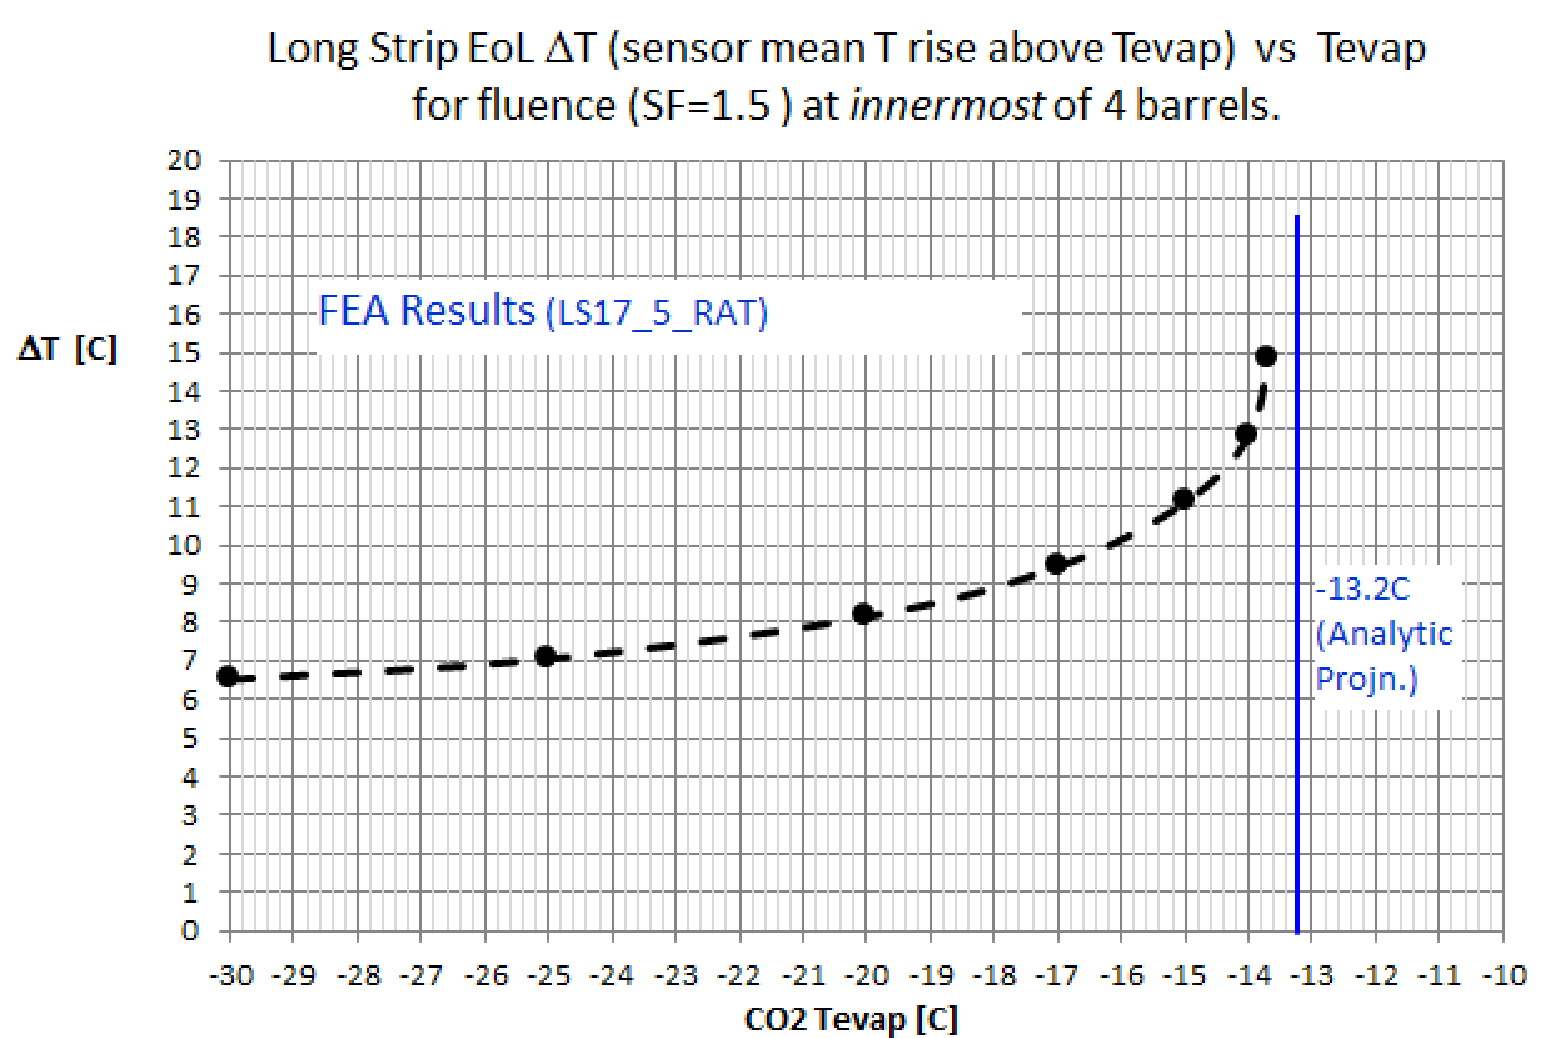
\includegraphics[width=0.4\linewidth]{figures/verification.pdf}
\caption{Thevenin equivalent of the thermal network (left). Result of surface temperature calculations using FEA (middle). Average temperature above cooling - comparison between FEA (dots) and network model prediction (right).}
\label{fig:modulerampperformance}
\end{figure}
